\usetikzlibrary{arrows}
\definecolor{aqaqaq}{rgb}{0.65,0.65,0.65}
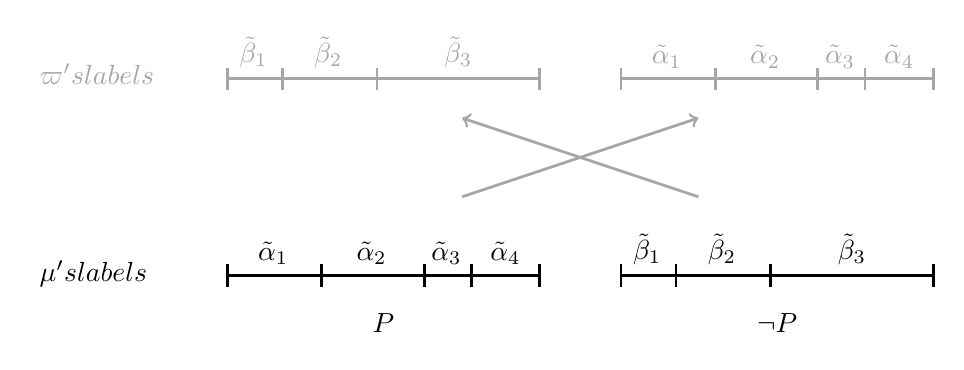
\begin{tikzpicture}[line width =1pt]%[line cap=round,line join=round,>=triangle 45,x=1cm,y=1cm]
%\clip(-2.5,-2.15) rectangle (9.7,5.1);

\draw (-2.5,0.32) node[anchor=north west] {$\mu\text{'s labels}$};

\draw (0,0) -- (4,0) node[midway, below = 10pt]{$P$};
\draw [|-] (0,0) -- (1.2,0) node[midway, above]{$\small\tilde{\alpha}_1$};
\draw [|-] (1.2,0) -- (2.5,0) node[midway, above]{$\small\tilde{\alpha}_2$};
\draw [|-] (2.5,0) -- (3.1,0) node[midway, above]{$\small\tilde{\alpha}_3$};
\draw [|-|] (3.1,0) -- (4,0) node[midway, above]{$\small\tilde{\alpha}_4$};

\draw (5,0) -- (9,0) node[midway, below = 10pt]{$\lnot P$};
\draw [|-] (5,0) -- (5.7,0) node[midway, above]{$\small\tilde{\beta}_1$};
\draw [|-] (5.7,0) -- (6.9,0) node[midway, above]{$\small\tilde{\beta}_2$};
\draw [|-|] (6.9,0) -- (9,0) node[midway, above]{$\small\tilde{\beta}_3$};

\begin{scope}[color = aqaqaq]
\draw (-2.5,2.82) node[anchor=north west] {$\varpi\text{'s labels}$};

\draw [|-] (0,2.5) -- (0.7,2.5) node[midway, above]{$\small\tilde{\beta}_1$};
\draw [|-] (0.7,2.5) -- (1.9,2.5) node[midway, above]{$\small\tilde{\beta}_2$};
\draw [|-|] (1.9,2.5) -- (4,2.5) node[midway, above]{$\small\tilde{\beta}_3$};

\draw [|-] (5,2.5) -- (6.2,2.5) node[midway, above]{$\small\tilde{\alpha}_1$};
\draw [|-] (6.2,2.5) -- (7.5,2.5) node[midway, above]{$\small\tilde{\alpha}_2$};
\draw [|-] (7.5,2.5) -- (8.1,2.5) node[midway, above]{$\small\tilde{\alpha}_3$};
\draw [|-|] (8.1,2.5) -- (9,2.5) node[midway, above]{$\small\tilde{\alpha}_4$};

\draw [->] (6,1) -- (3,2);
\draw [->] (3,1) -- (6,2);
\end{scope}

\end{tikzpicture}